%\documentclass{beamer}

\documentclass[xcolor=dvipsnames]{beamer}
\usepackage{tikz}
\usepackage{beamerthemesplit}
\usepackage{pdfpages}
\usepackage{tikz}
\usepackage{xcolor}
%\documentclass[10pt]{beamer}
%\documentclass[xcolor=dvipsnames]{beamer}
\usetheme{Madrid}
%\definecolor{Farbe}{rgb}{0.04706, 0.13725, 0.26667}
\usecolortheme[named=Cyan]{structure}
%\usecolortheme{beaver}
\usepackage[utf8]{inputenc}
\usepackage{amsmath}
\usepackage{amsfonts}
\usepackage{amssymb}
\usepackage{float}
\usepackage{multicol}
\usepackage{graphicx}
\usepackage{color}
\usepackage{caption}
\usepackage{subcaption}
\usepackage{hyperref}
\usepackage{flexisym}
\begin{document}
		\title{Efficiency of SVD in phase-II }
		   
		\author{Soumen Halder} 
		\date{\today} 
			\subtitle{ SVD general meeting }
		\frame{\titlepage}
		
\begin{frame}{Software}
	\begin{itemize}
		\item \textbf{hlt\_mumu\_2trk} skim raw data used from KEKCC(/ghi/fs01/belle2/bdata/Data/release-02-00-01/DB00000425/prod00000005/e0003/4S/r*/all/raw/sub00/\\raw.physics.hlt\_mumu\_2trk*) 
		\item \textbf{hlt\_bhabha} skim raw data used from KEKCC(/ghi/fs01/belle2/bdata/Data/release-02-00-01/DB00000425/prod00000005/e0003/4S/r*/all/raw/sub00/\\raw.physics.hlt\_bhabha*) 
		\item The runs without SVD were excluded from analysis
		\item Details of skim discussed here \\ \url{https://confluence.desy.de/display/BI/Experiment+3+skims}
		\item DR2 dimuon sample used as MC sample
		\item Release used to analysis is \textbf{/cvmfs/belle.cern.ch/sl6/releases/releases-02-00-01}
	\end{itemize}
\end{frame}
		\begin{frame}{Further Selection criteria applied }
			For dimuon
			\begin{itemize}
				\item \# of tracks=2
				\item $35^{\circ}<\theta<125^{\circ}$
				\item acollinearity$<10^{\circ}$
				\item 0 GeV$<$EClenergy$<0.7$GeV
				\item $|d_0|<2$ cm and $|z_0|<4$ cm		
			\end{itemize}
				For Bhabha
				\begin{itemize}
					\item \# of tracks=2
					
					\item acollinearity$<10^{\circ}$
				    \item Momentum of each of two tracks $>$ 3GeV 
					\item $|d_0|<2$ cm and $|z_0|<4$ cm		
				\end{itemize}
		\end{frame}

\begin{frame}{Finding residual}
	\begin{multicols}{2}
		\begin{itemize}
			\item  Fit track without the clusters of a layer for which residual wish to calculate(to remove biasness)
			\item \textbf{ Residual = (SVD\_Cluster\_position -- SVD\_Intercept\_position)}\\
			where SVD\_Intercept\_position is position of extrapolation of track to SVD		
		\end{itemize}
		\begin{figure}[H]		
			\begin{center}
				\begin{subfigure}[b]{0.30\textwidth}
					%                \centering
					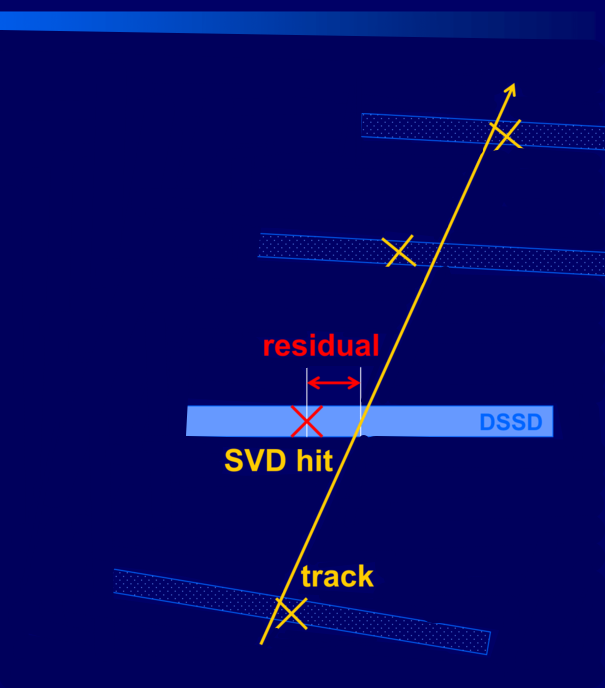
\includegraphics[width=4.5cm]{hit.png}
				\end{subfigure}\\
			\end{center}
		\end{figure}
	\end{multicols}		
\end{frame}
\begin{frame}{Residual plot and efficiency}

		\begin{itemize}
			\item[1)] Loop on SVD\_Intercepts
			\item[2)] Continue the loop if it does not satisfy following criteria
			\begin{itemize}
			\item[$=>$] the intercept is within 10 strips from sensor edge
			\item[$=>$] the intercept having at least  one pxd hit and at least two svd hits
			\end{itemize}
		\begin{itemize}
				
				\item[i)]Loop on all the clusters(which are inside ROIs) in the event and 
				\begin{itemize}
					\item[$->$] If layer, ladder, sensor matches with SVD\_Intercept then residual calculated as \textbf{ Residual = (SVD\_Cluster\_position -- SVD\_Intercept\_position)} 
					\item[$->$] For multiple clusters on same sensor, same side(U/V) that cluster is taken as an entry of residual plot  for which residual is minimum				   
				\end{itemize}		
			\end{itemize} 					
		\end{itemize}
		\begin{itemize}
			\item Efficiency=$\frac{\text{\# of cluster within }\pm0.05 cm\text{ in residual plot}}{\text{\# of intercepts}}$			
		\end{itemize}
N.B: size of roi is 2.5x2.5 $\text{cm}^2$

\end{frame}
 \begin{frame}{Intercept V\_coordinate vs U\_coordinate}
 	For dimuon data
 	\begin{multicols}{4}	
 		\begin{figure}[H]
 			\begin{center}				
 				\begin{subfigure}[b]{0.30\textwidth}
 					%                \centering
 					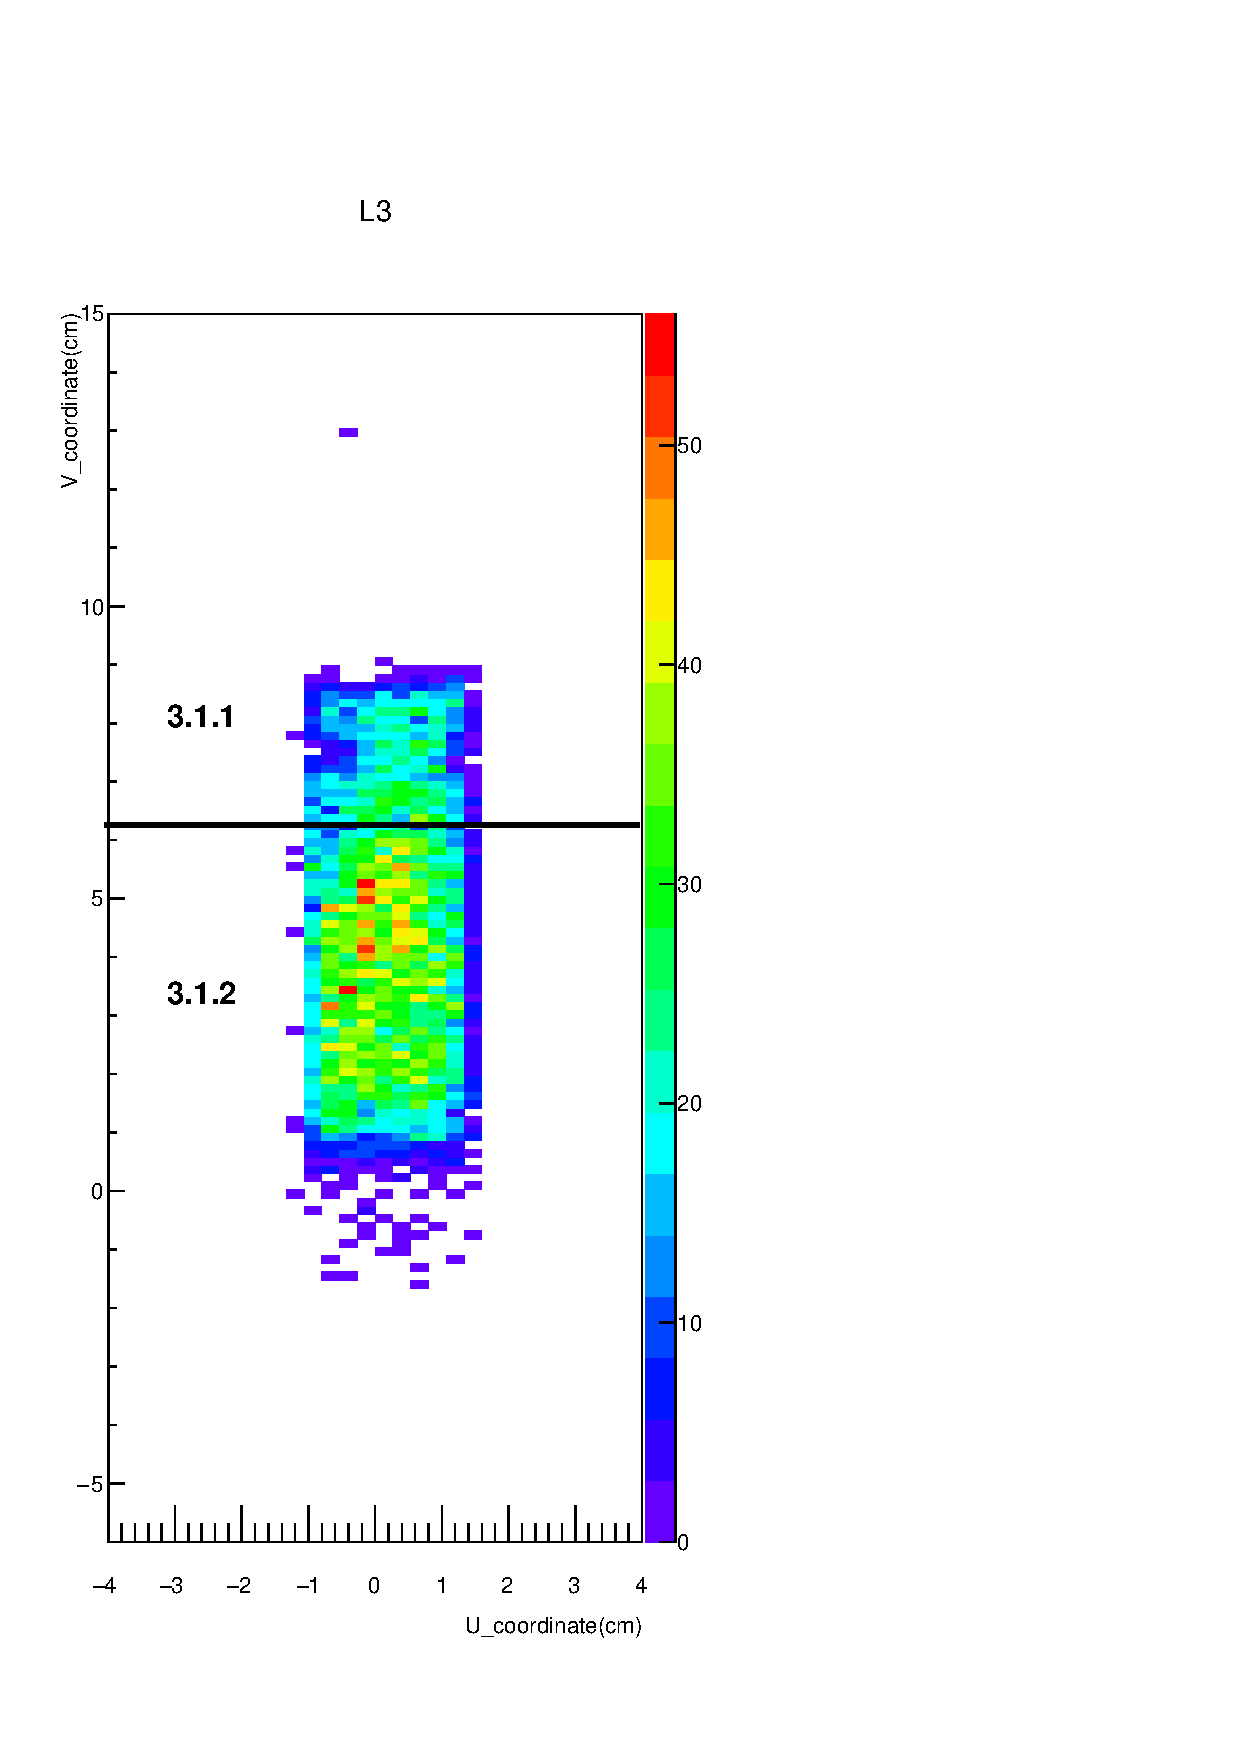
\includegraphics[width=2cm]{L3uv.pdf}
 					\caption*{L3}
 				\end{subfigure}				
 			\end{center}
 		\end{figure}
 		\begin{figure}[H]
 			\begin{center}				
 				\begin{subfigure}[b]{0.30\textwidth}
 					%                \centering
 					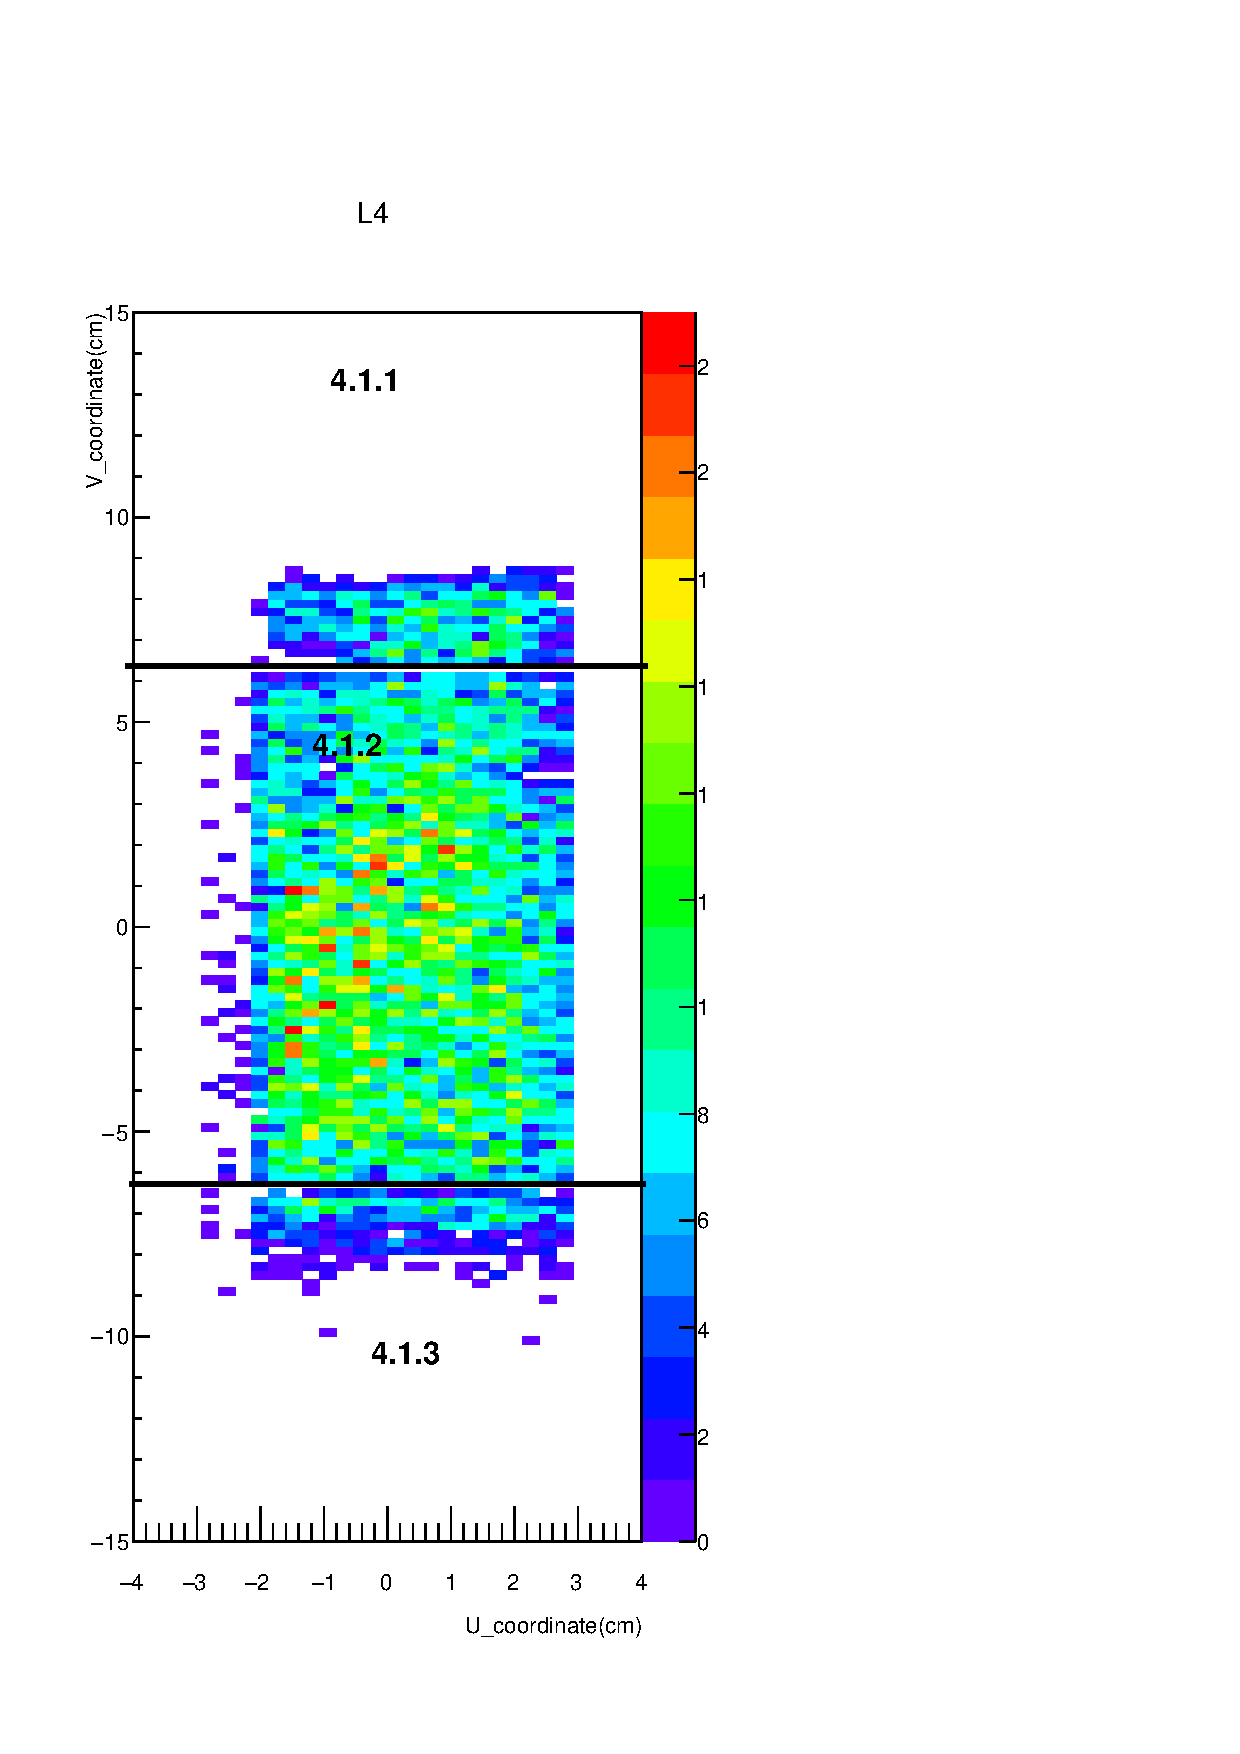
\includegraphics[width=2cm]{L4uv.pdf}
 				\end{subfigure}		
 				\caption*{L4}		
 			\end{center}
 		\end{figure}
 		\begin{figure}[H]
 			\begin{center}				
 				\begin{subfigure}[b]{0.30\textwidth}
 					%                \centering
 					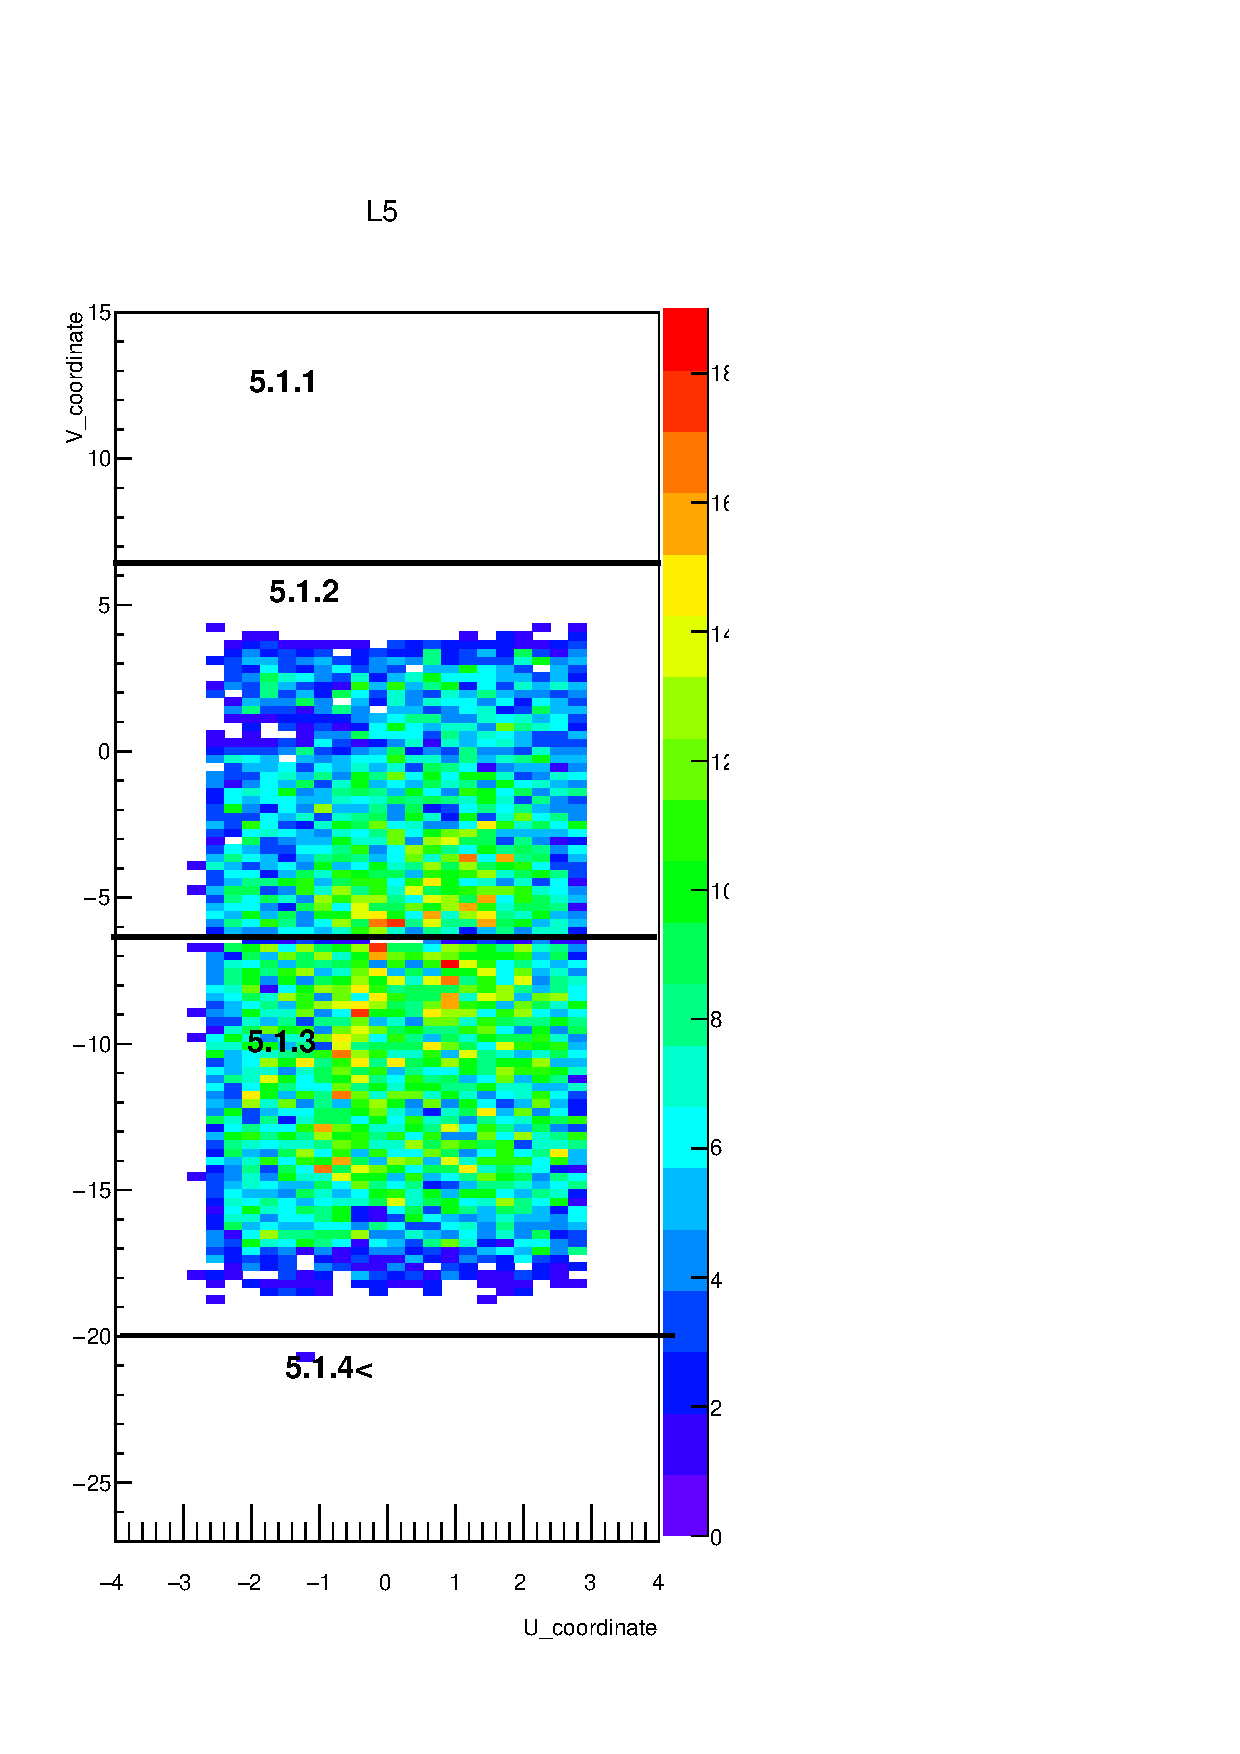
\includegraphics[width=2cm]{L5uv.pdf}
 				\end{subfigure}		
 				\caption*{L5}		
 			\end{center}
 		\end{figure}
 		\begin{figure}[H]
 			\begin{center}				
 				\begin{subfigure}[b]{0.30\textwidth}
 					%                \centering
 					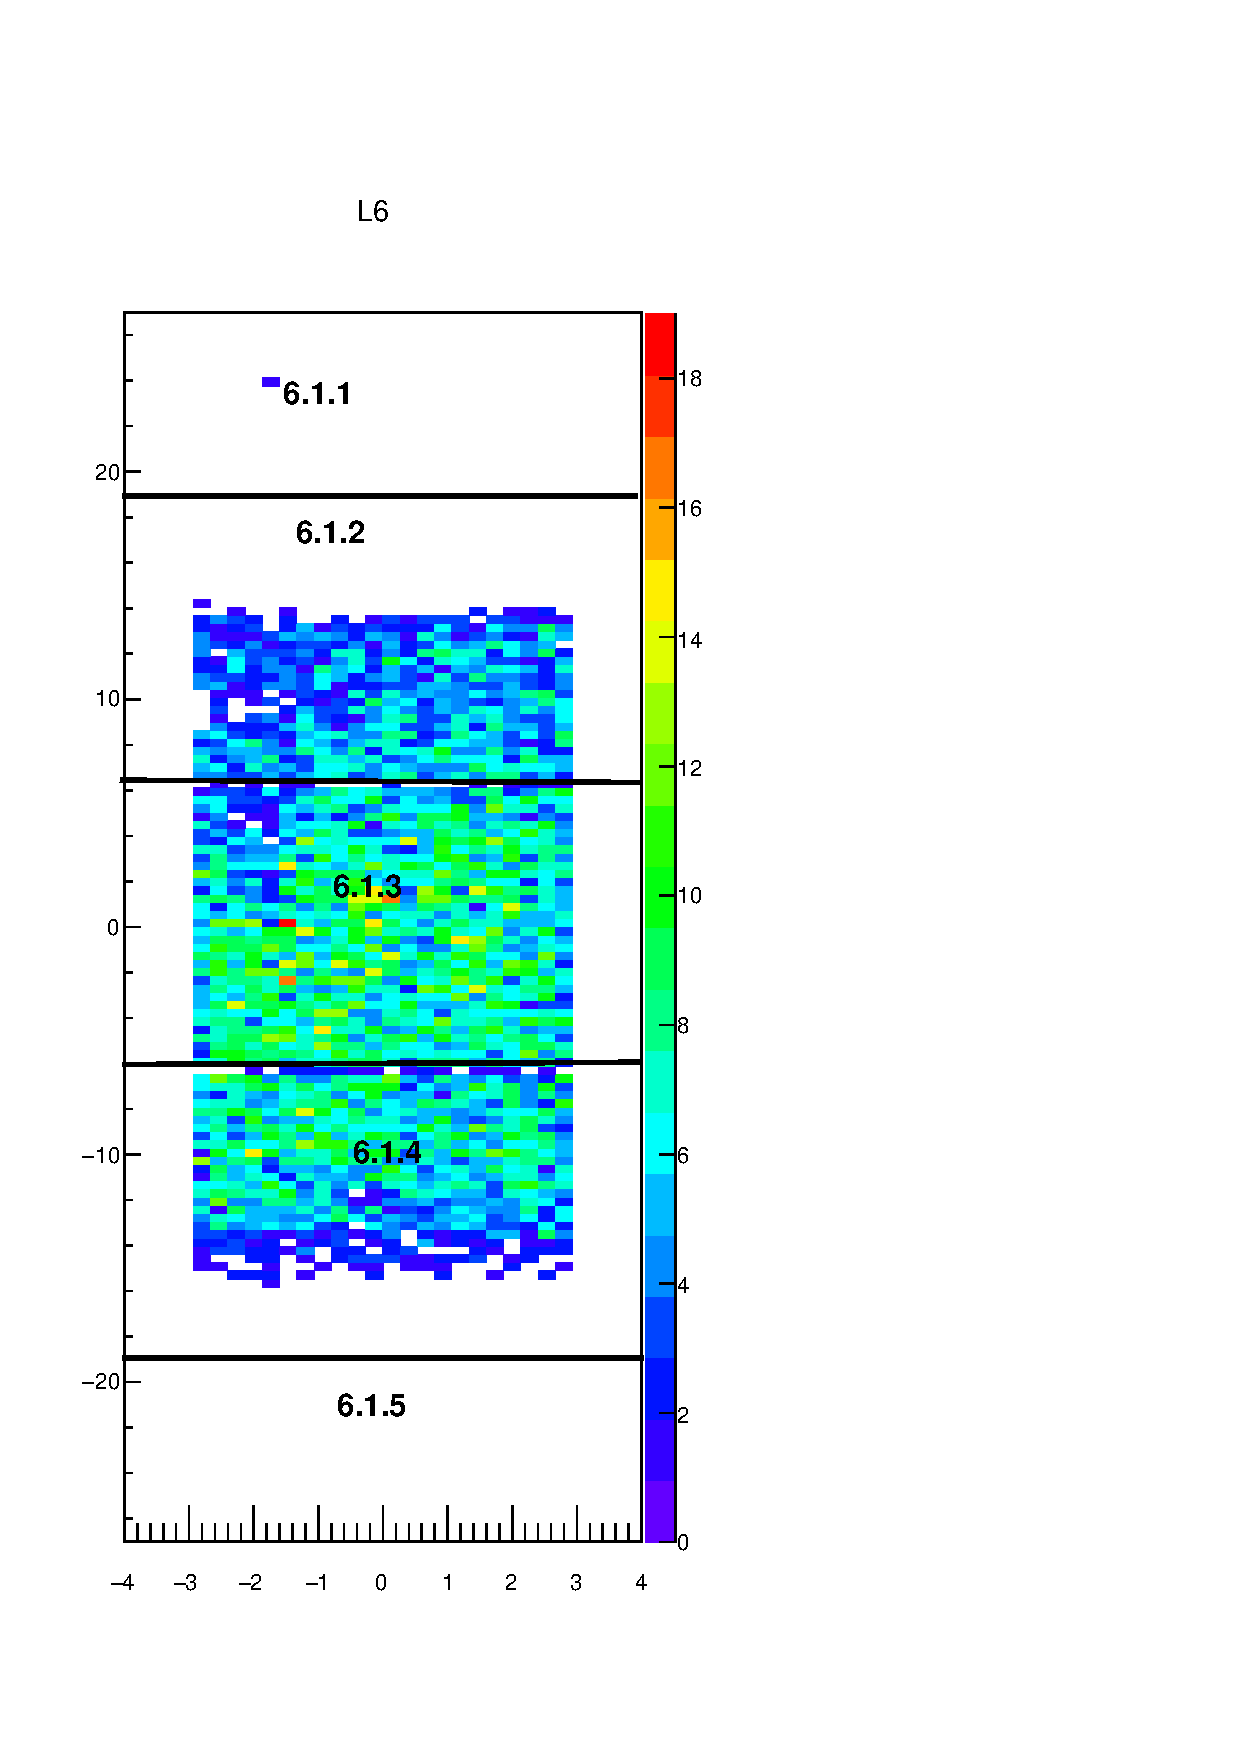
\includegraphics[width=2cm]{L6uv.pdf}
 				\end{subfigure}		
 				\caption*{L6}		
 			\end{center}
 		\end{figure}
 	\end{multicols}	
 	
 \end{frame}
 \begin{frame}{Intercept V\_coordinate vs U\_coordinate}
 	For Bhabha data
 	\begin{multicols}{4}	
 		\begin{figure}[H]
 			\begin{center}				
 				\begin{subfigure}[b]{0.30\textwidth}
 					%                \centering
 					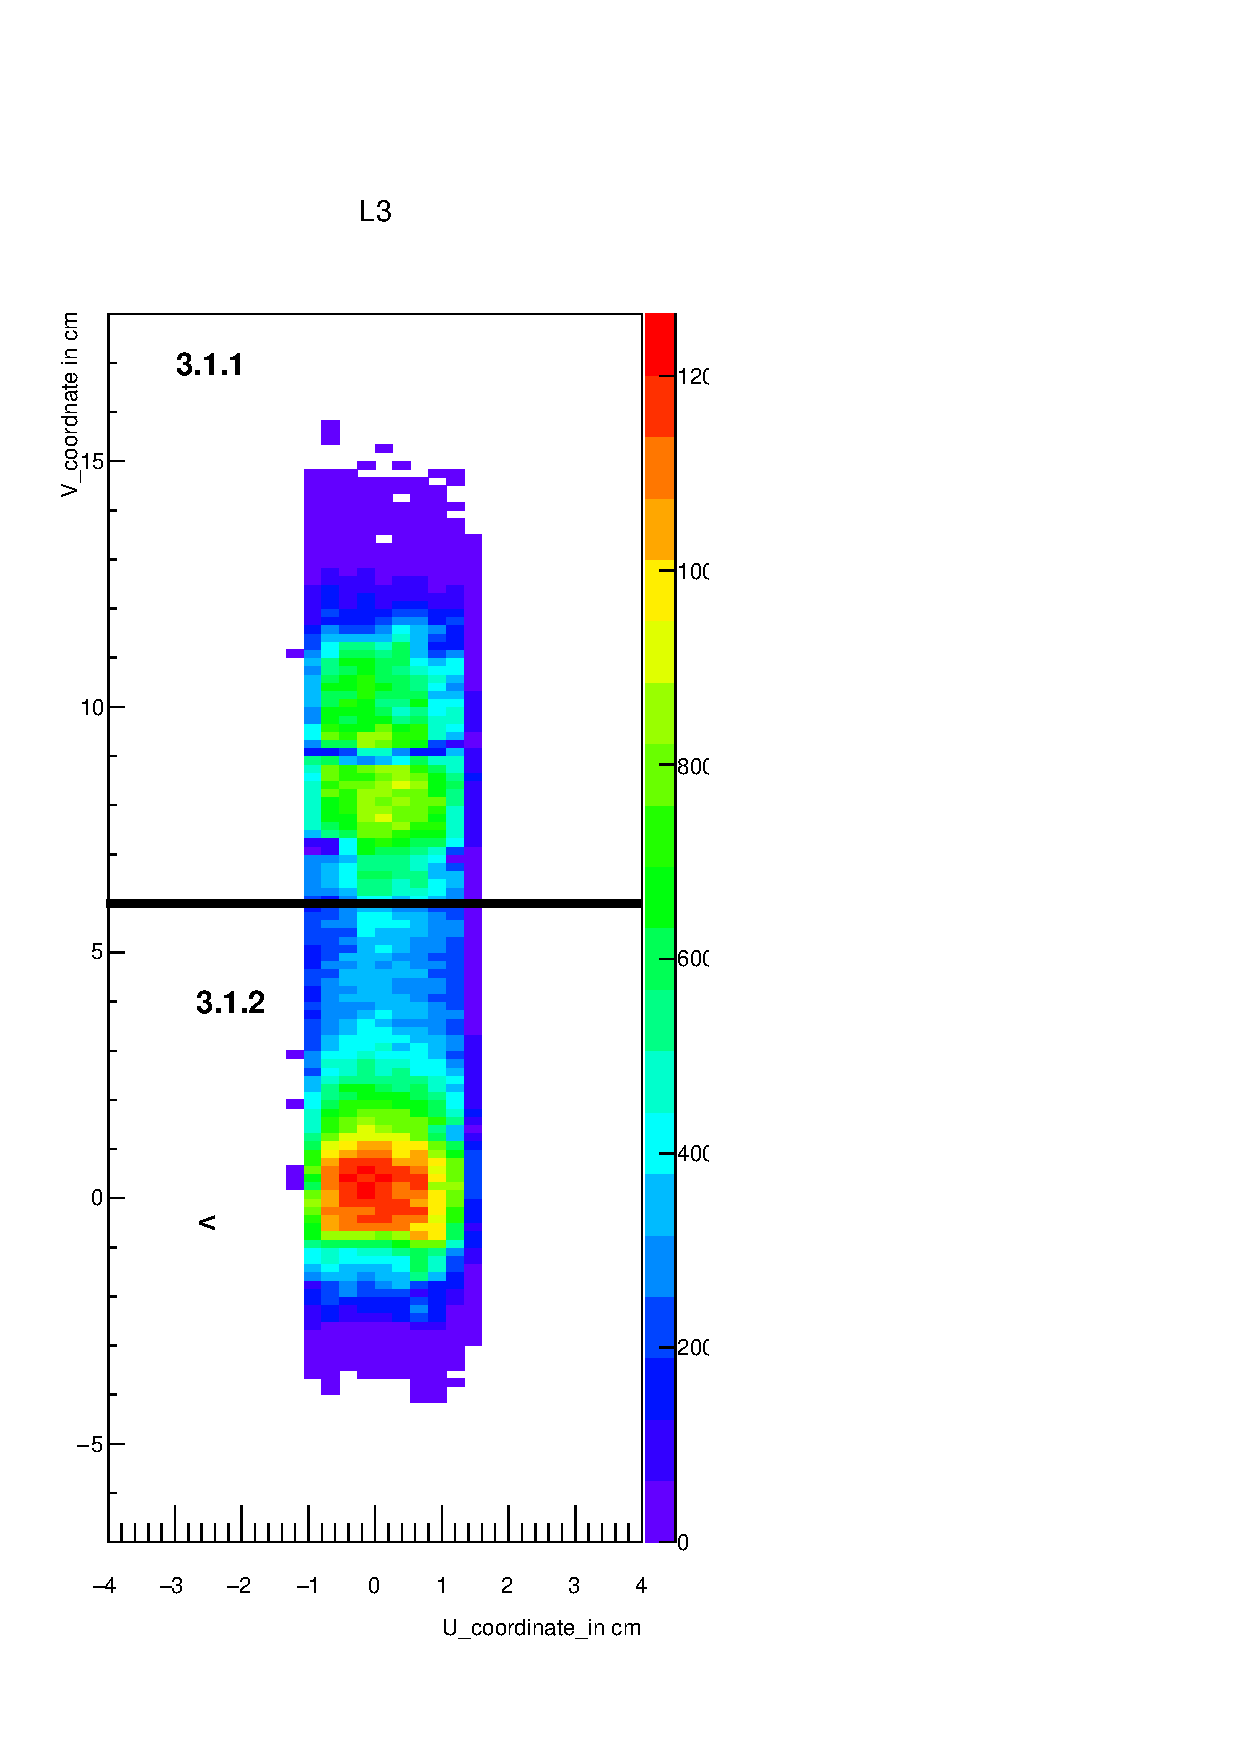
\includegraphics[width=2cm]{L3_bhabha.pdf}
 					\caption*{L3}
 				\end{subfigure}				
 			\end{center}
 		\end{figure}
 		\begin{figure}[H]
 			\begin{center}				
 				\begin{subfigure}[b]{0.30\textwidth}
 					%                \centering
 					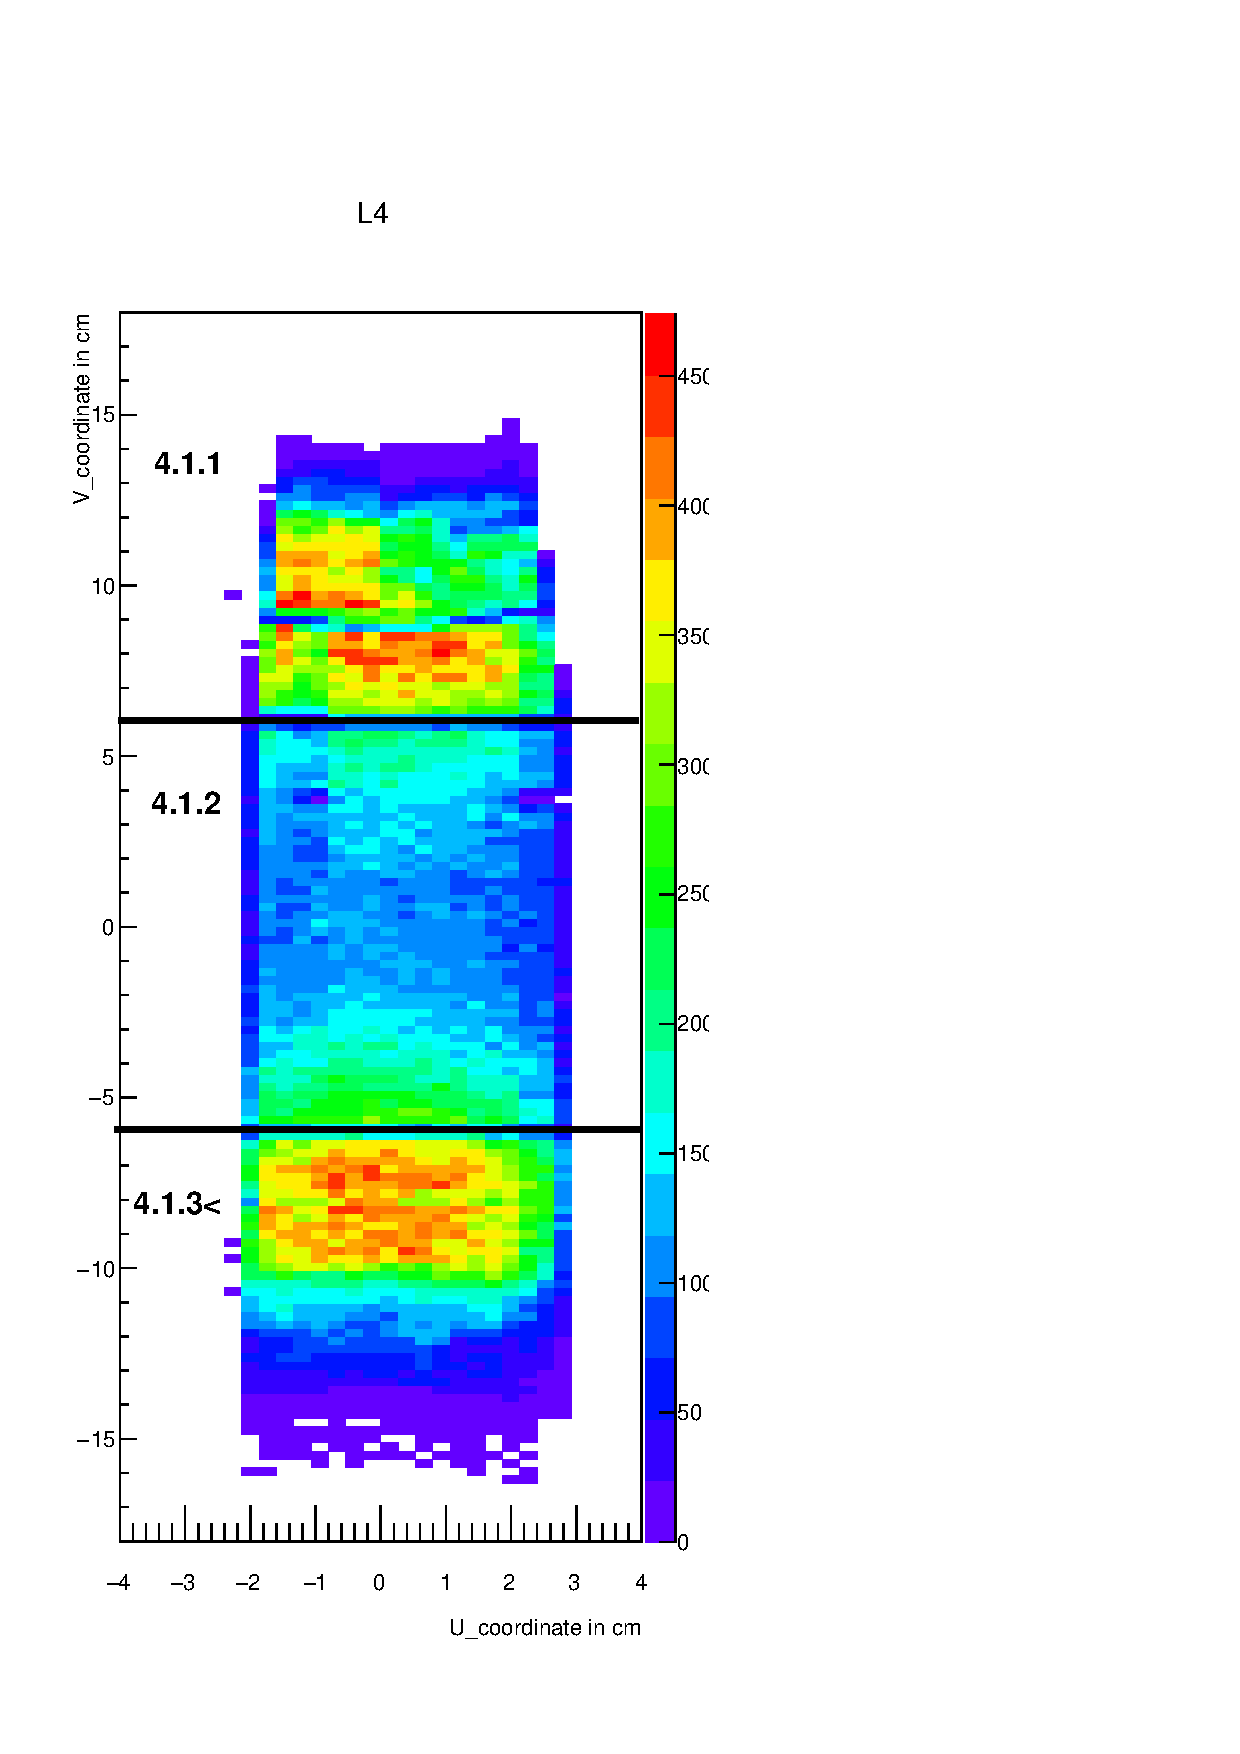
\includegraphics[width=2cm]{L4_bhabha.pdf}
 				\end{subfigure}		
 				\caption*{L4}		
 			\end{center}
 		\end{figure}
 		\begin{figure}[H]
 			\begin{center}				
 				\begin{subfigure}[b]{0.30\textwidth}
 					%                \centering
 					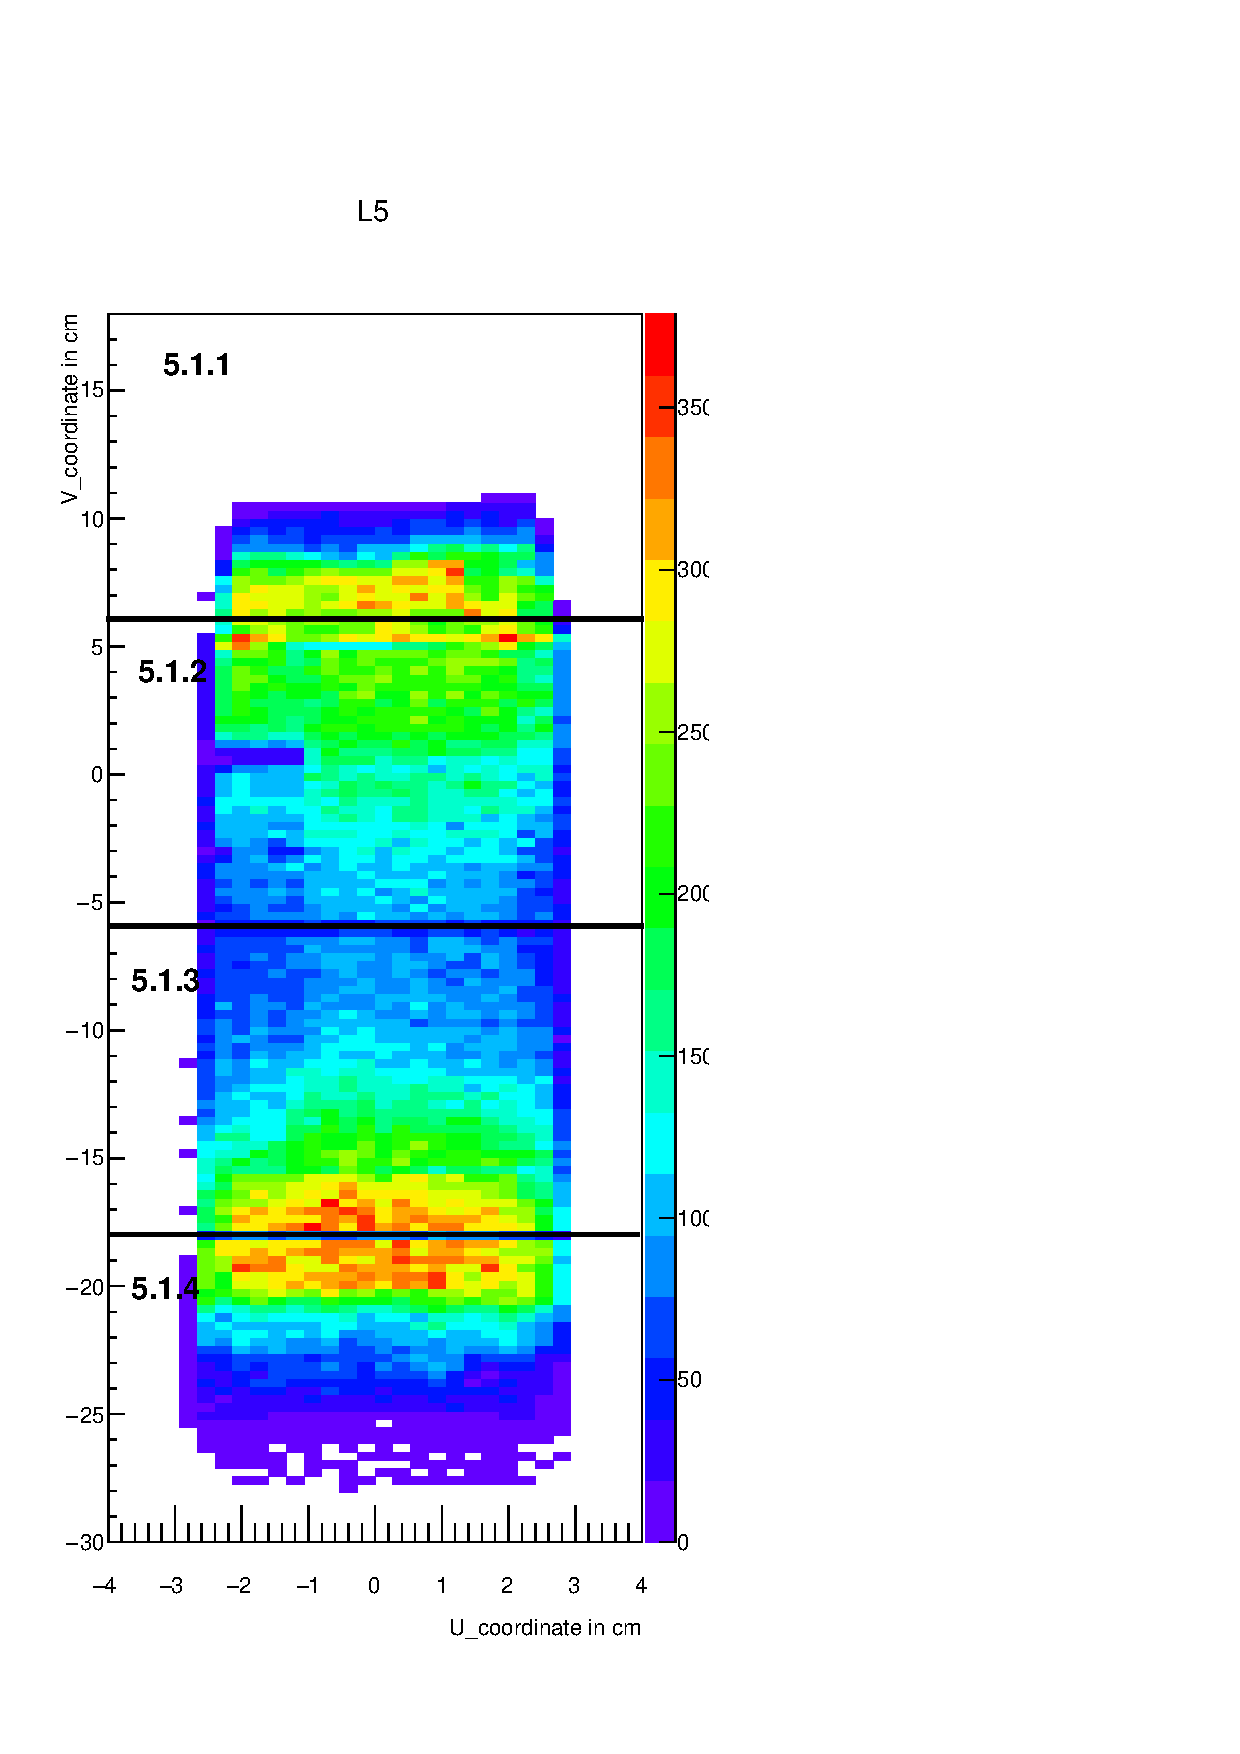
\includegraphics[width=2cm]{L5_bhabha.pdf}
 				\end{subfigure}		
 				\caption*{L5}		
 			\end{center}
 		\end{figure}
 		\begin{figure}[H]
 			\begin{center}				
 				\begin{subfigure}[b]{0.30\textwidth}
 					%                \centering
 					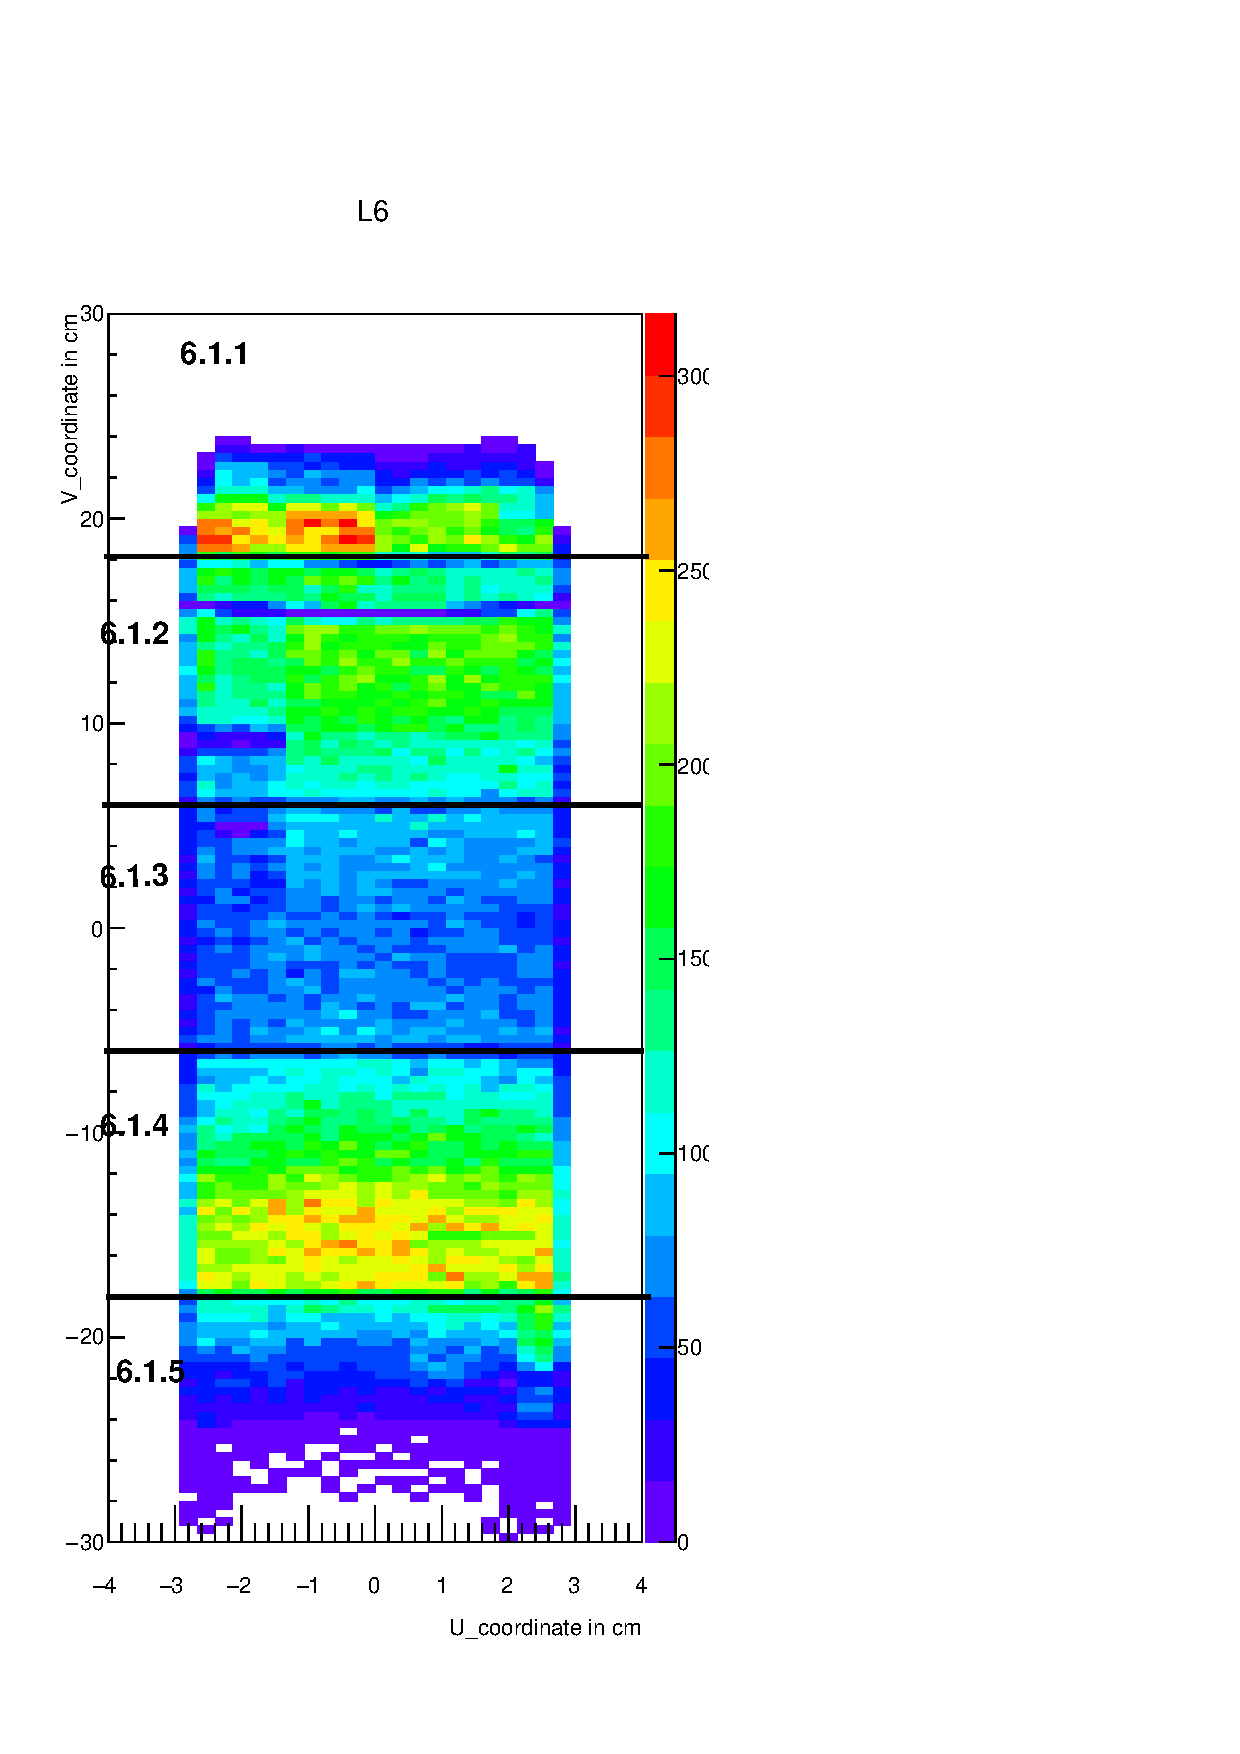
\includegraphics[width=2cm]{L6_bhabha.pdf}
 				\end{subfigure}		
 				\caption*{L6}		
 			\end{center}
 		\end{figure}
 	\end{multicols}	
 	
 \end{frame}
 
 \begin{frame}
 	
 	
 	\begin{center}	
 		\begin{tabular}{|c|c|c| c|c|c|}
 			\hline
 			
 			Layer &	\multicolumn{5}{|c|}{Efficiency for }	\\ 
 			\cline{2-6}
 			Ladder &\multicolumn{1}{|c|}{MC dimuon }&\multicolumn{2}{|c|}{Data dimuon }&\multicolumn{2}{|c|}{Data bhabha }	\\ \cline{2-6} 			
 			sensor &&&modified&&modified\\
 			side &&&&&\\ \cline{2-6}	
 			\hline
 		311U &   0.9971  & 0.9860  &           &  0.9911 &          \\          
 		311V &   0.9978  & 0.9973  &           &  0.9960 &          \\  
 		312U &   0.9978  & 0.9885  &           &  0.9911 &          \\  
 		312V &   0.9985  & 0.9905  &           &  0.9916 &          \\  
 		\hline
 		411V &   0.9990  & 0.9986  &           &  0.9952 &          \\  
 		412U &   0.9992  & 0.7909  & 0.9930    &  0.8076 & 0.9850   \\  
 		412V &   0.9991  & 0.9738  &           &  0.9749 &          \\  
 		413U &   0.9995  & 0.9919  &           &  0.9954 &          \\  
 		413V &   0.9993  & 1.0     &           &  0.9961 &          \\  
 		
 		\hline
 		511V &   --      & --      &           &  0.9803 &          \\  
 		512U &   0.9995  & 0.8493  &  0.9877   &  0.8466 &  0.9913  \\  
 		512V &   0.9989  & 0.9931  &           &  0.9826 &          \\
 				  
 				\end{tabular}
 				
 			\end{center}
 			
 		\end{frame}
 			
 		\begin{frame}
 			
 			
 			\begin{center}	
 				\begin{tabular}{|c|c|c| c|c|c|}
 					\hline
 					
 					Layer &	\multicolumn{5}{|c|}{Efficiency for }	\\ 
 					\cline{2-6}
 					Ladder &\multicolumn{1}{|c|}{MC dimuon }&\multicolumn{2}{|c|}{Data dimuon }&\multicolumn{2}{|c|}{Data bhabha }	\\ \cline{2-6} 			
 					sensor &&&modified&&modified\\
 					side &&&&&\\ \cline{2-6}	
 					\hline	
 	513U &   0.9994  & 0.9828  &           &  0.9851 &          \\  
 	513V &   0.9993  & 0.9402  &           &  0.9582 &          \\  
 	514U &   --      & --      &           &  0.9982 &          \\  
 	514V &   --      & --      &           &  0.9952 &          \\  
 	\hline
 	
 	611V &   --      & --      &           &  0.9960 &          \\  
 	612U &   0.9994  & 0.8671  &  0.9943   &  0.8529 &  0.9961  \\  
 	612V &   0.9991  & 0.9876  &           &  0.9813 &          \\  
 	613U &   0.9996  & 0.8287  &  0.9877   &  0.8323 &  0.9872  \\  
 	613V &   0.9995  & 0.9936  &           &  0.9935 &          \\  
 	614U &   0.9996  & 0.9836  &           &  0.9818 &          \\  
 	614V &   0.9995  & 0.9902  &           &  0.9854 &          \\  
 	615U &   --      & --      &           &  0.9972 &          \\  
 	615V &   --	 & --      &           &  0.9949 &           \\  
 	\hline
 		\end{tabular}
 		
 	\end{center}
 	
 \end{frame}


\begin{frame} {Cluster position distribution}
	\begin{multicols}{2}
		\begin{figure}[H]
			\begin{center}			
				\begin{subfigure}[b]{0.40\textwidth}
					%                \centering
					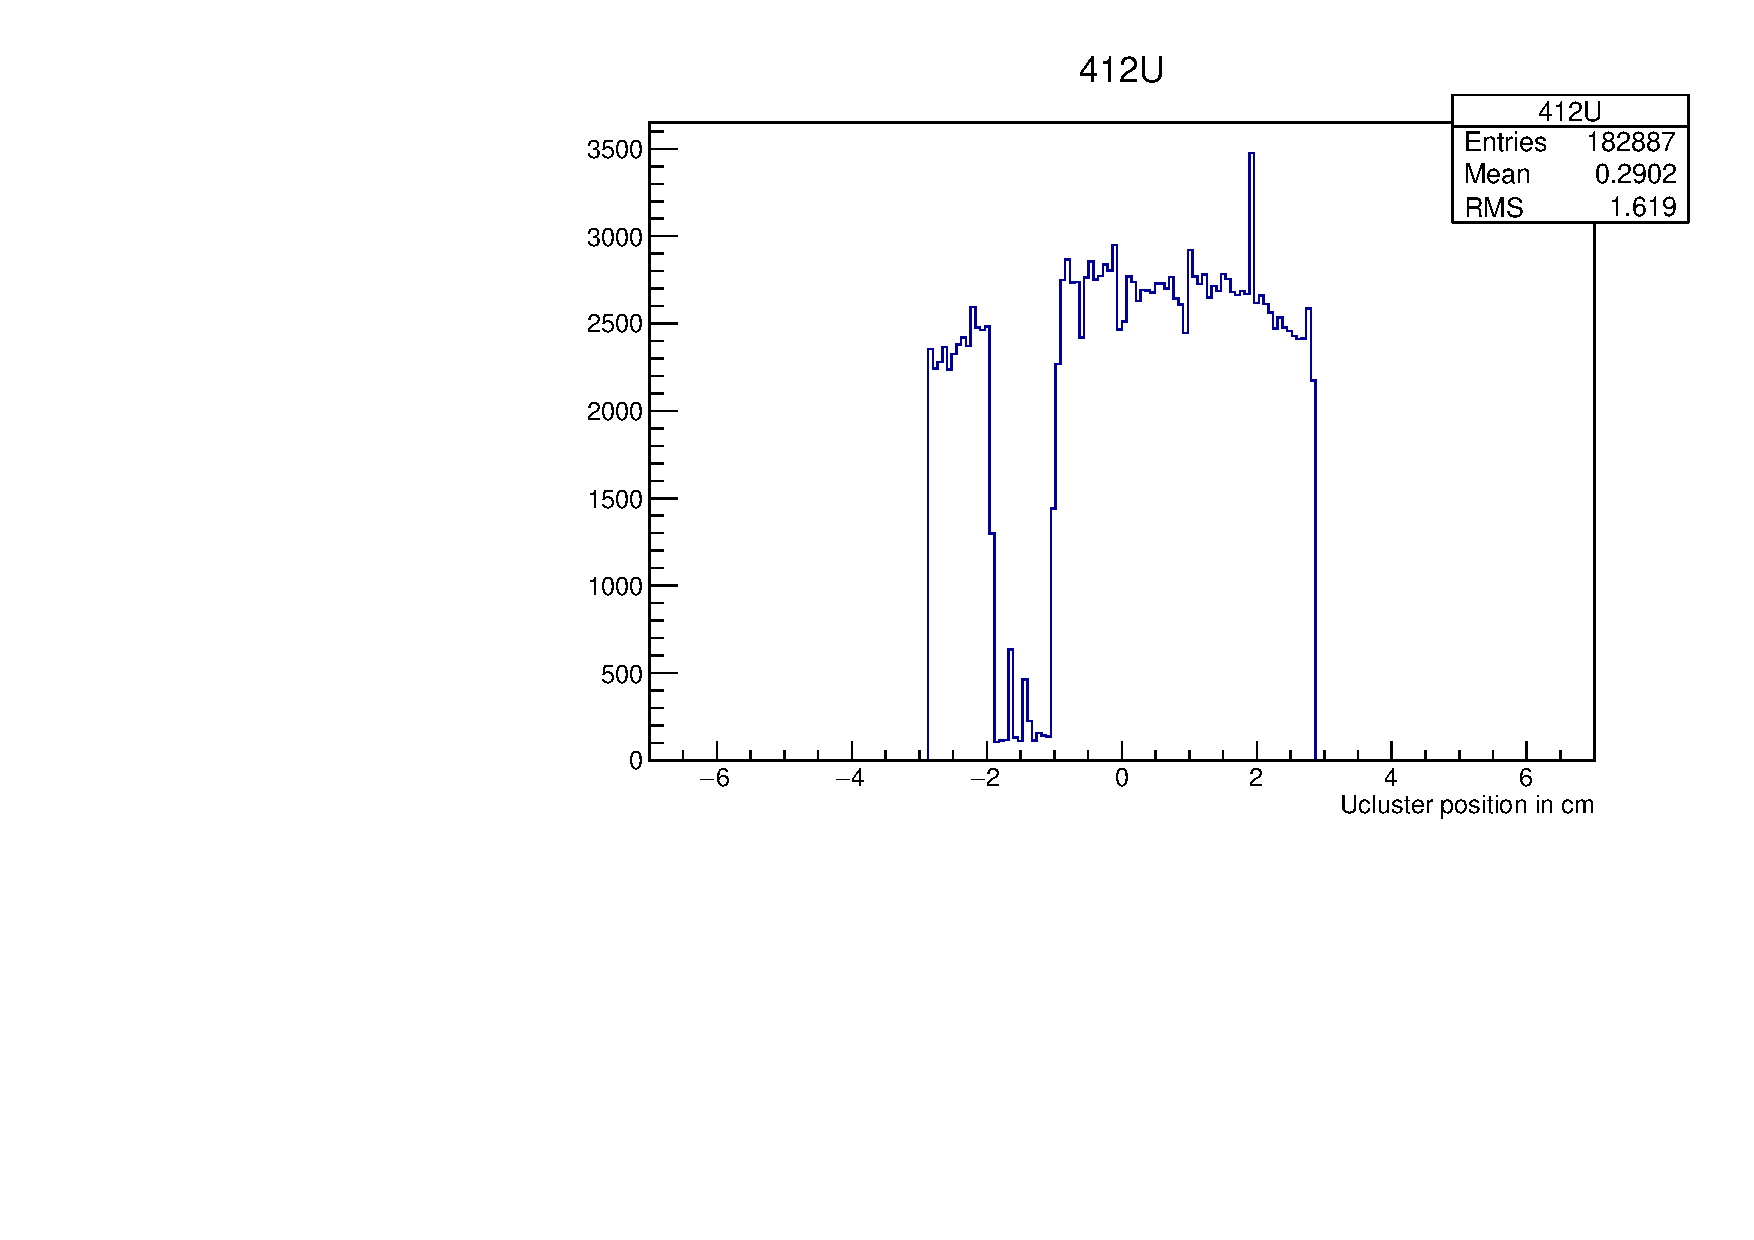
\includegraphics[width=5cm]{412U.pdf}
				\end{subfigure}						
			\end{center}
		\end{figure}
		\begin{figure}[H]
			\begin{center}			
				\begin{subfigure}[b]{0.40\textwidth}
					%                \centering
					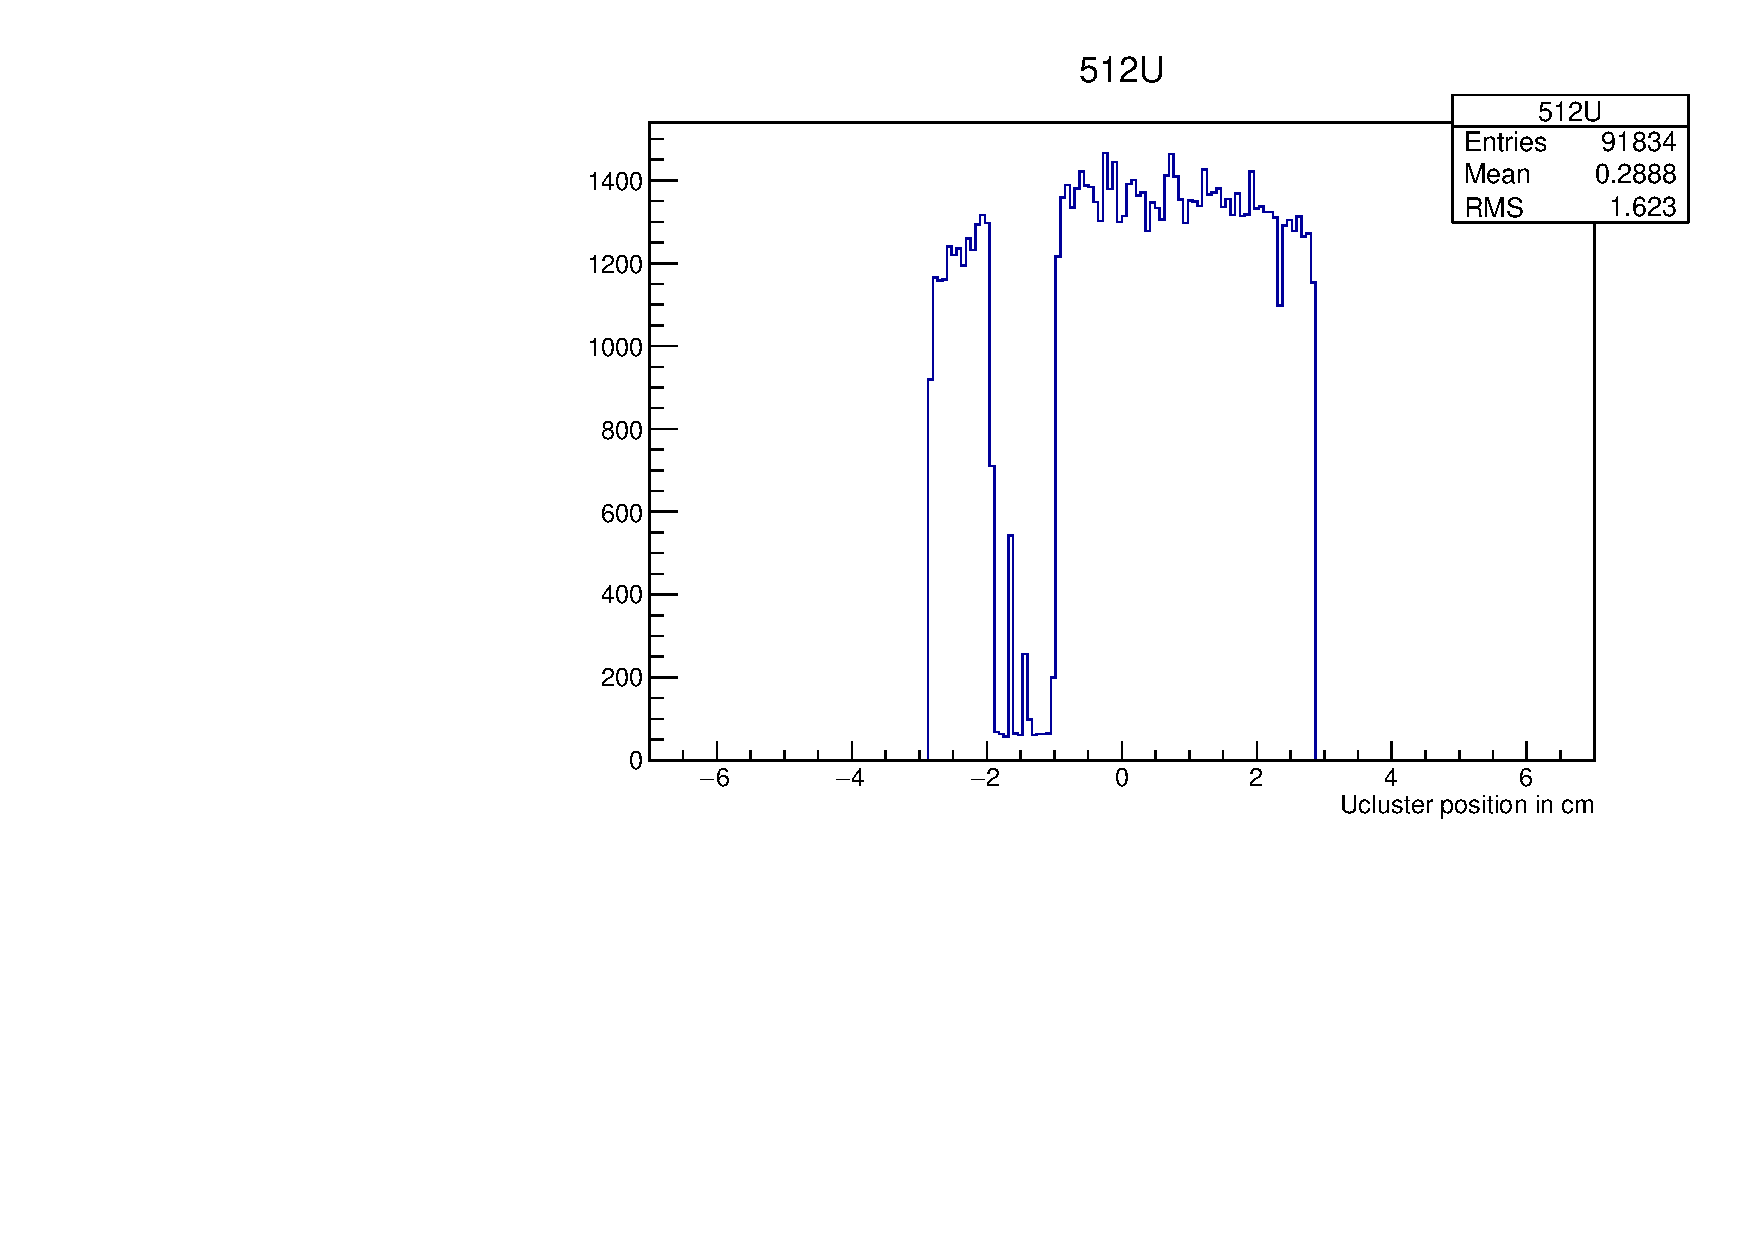
\includegraphics[width=5cm]{512U.pdf}
				\end{subfigure}				
			\end{center}
		\end{figure}
	\end{multicols} 
	\begin{multicols}{2}
		\begin{figure}[H]
			\begin{center}			
				\begin{subfigure}[b]{0.40\textwidth}
					%                \centering
					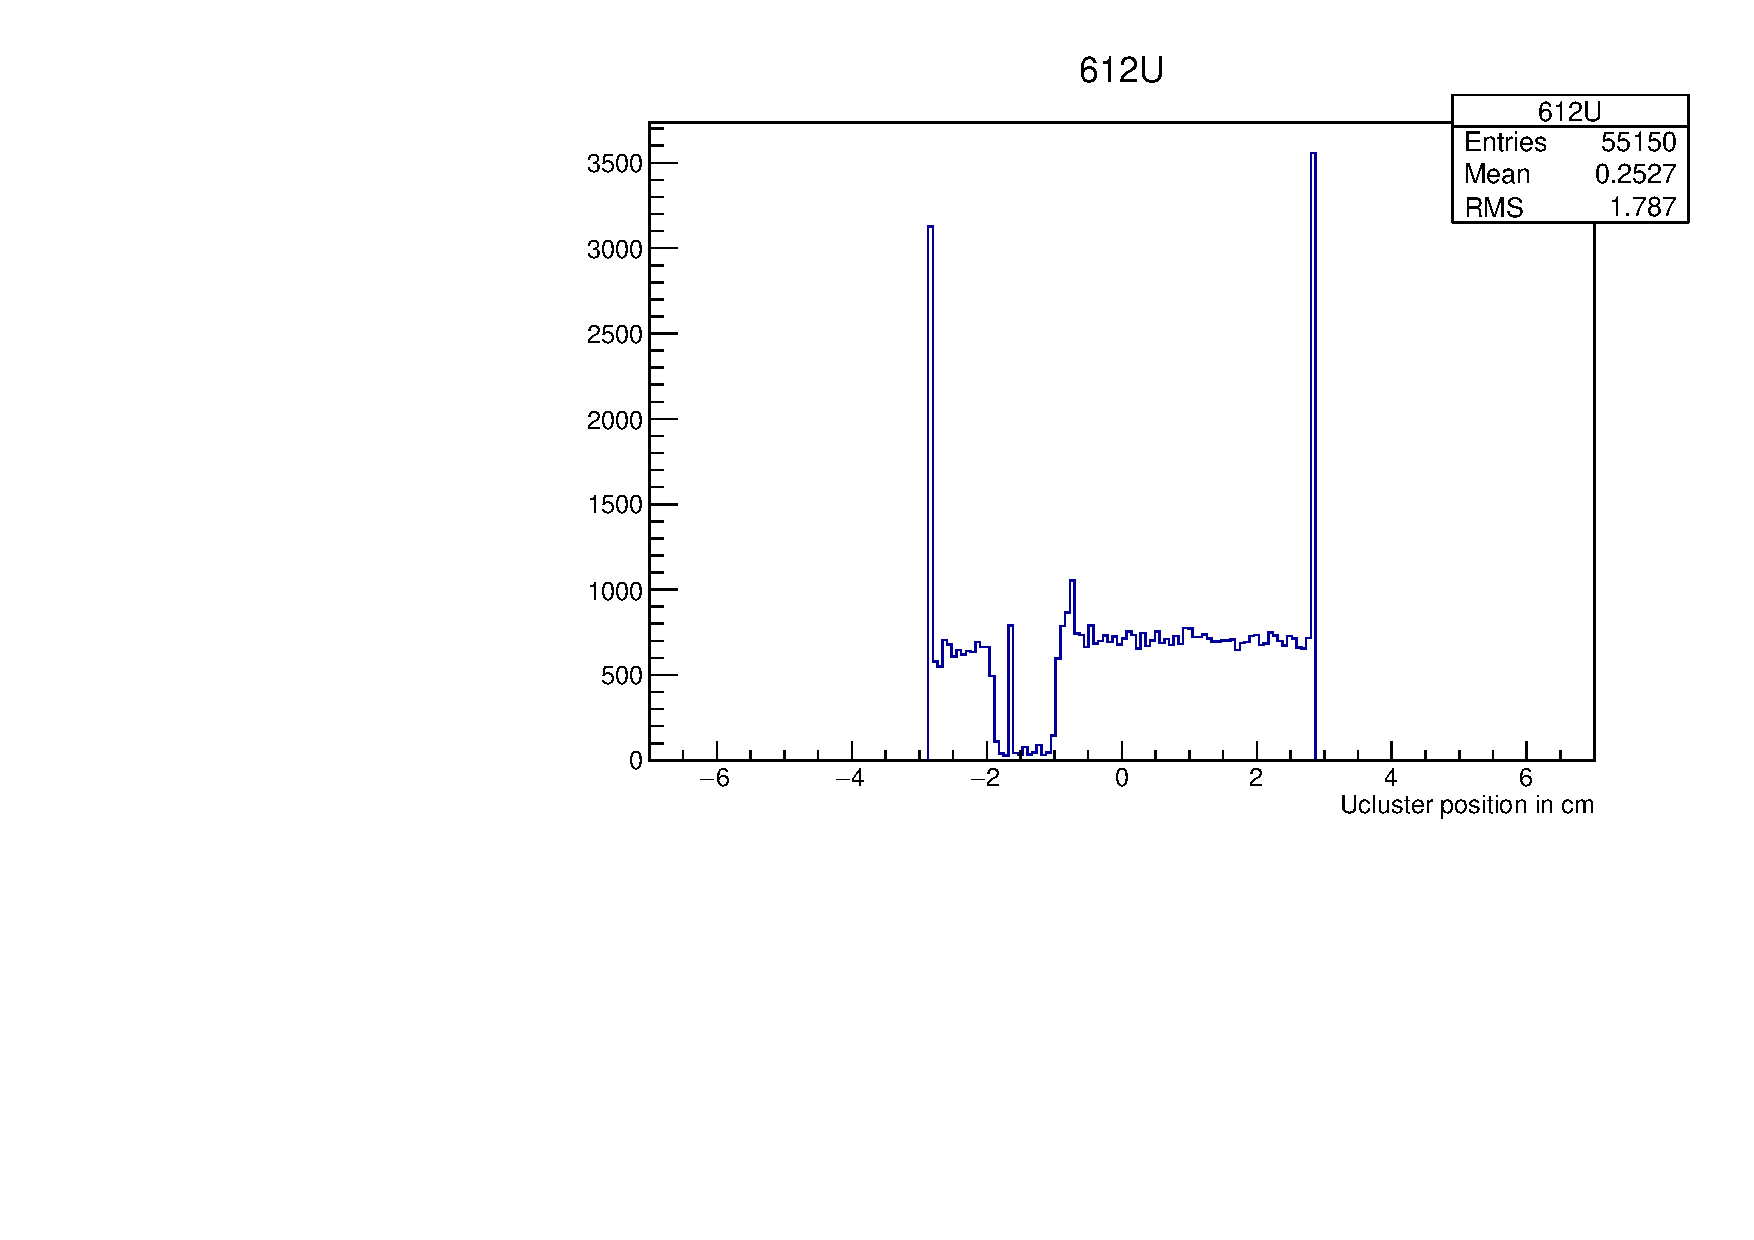
\includegraphics[width=5cm]{612U.pdf}
				\end{subfigure}						
			\end{center}
		\end{figure}
		\begin{figure}[H]
			\begin{center}			
				\begin{subfigure}[b]{0.40\textwidth}
					%                \centering
					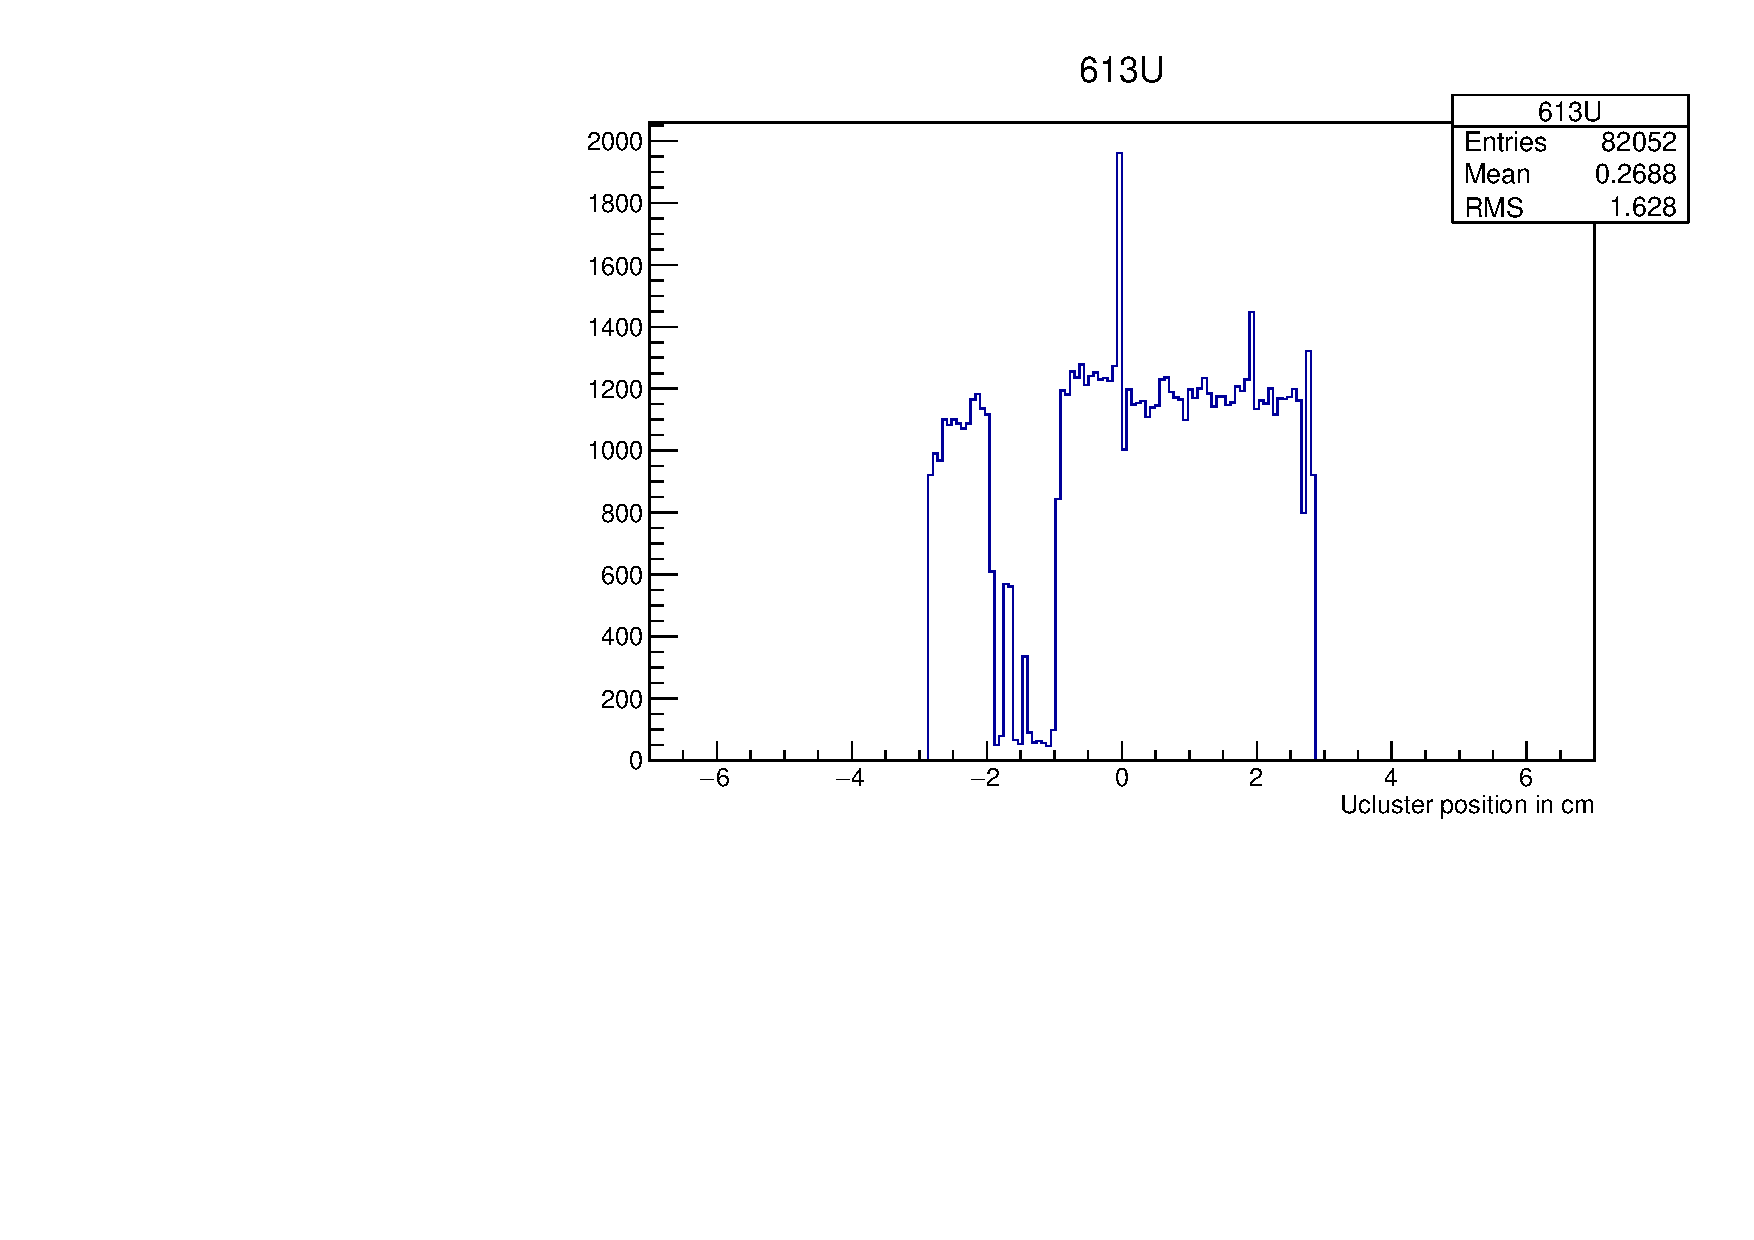
\includegraphics[width=5cm]{613U.pdf}
				\end{subfigure}				
			\end{center}
		\end{figure}
	\end{multicols}        
\end{frame}
\begin{frame}{Recalculating efficiency for above sensors}
	\begin{itemize}
		\item For above sensors one APV was masked for most of runs. That's why I have recalculated efficiency excluding intercepts having 108$<$u\_stripID$<$276. 
	\end{itemize}
\end{frame}
\begin{frame}{Conclusion}
	\begin{itemize}
		\item Without any apparent reason 513V has very low resolution
		\item Works going on to extract spatial resolution using phase-II data
	\end{itemize}
\end{frame}

\end{document}